% This file was created with tikzplotlib v0.10.1.
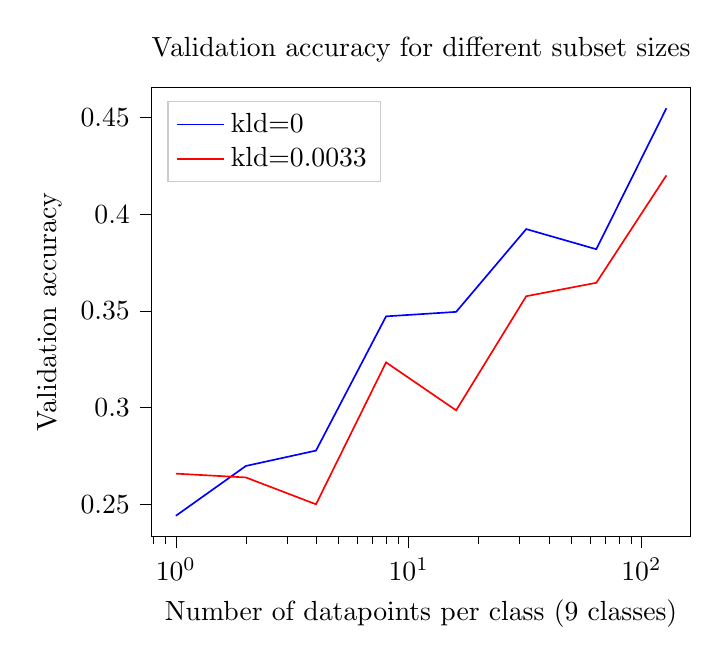
\begin{tikzpicture}

\definecolor{darkgray176}{RGB}{176,176,176}
\definecolor{lightgray204}{RGB}{204,204,204}

\begin{axis}[
legend cell align={left},
legend style={
  fill opacity=0.8,
  draw opacity=1,
  text opacity=1,
  at={(0.03,0.97)},
  anchor=north west,
  draw=lightgray204
},
log basis x={10},
tick align=outside,
tick pos=left,
title={Validation accuracy for different subset sizes},
x grid style={darkgray176},
xlabel={Number of datapoints per class (9 classes)},
xmin=0.784584097896751, xmax=163.143760296865,
xmode=log,
xtick style={color=black},
y grid style={darkgray176},
ylabel={Validation accuracy},
ymin=0.23350693488121, ymax=0.465401781729289,
ytick style={color=black}
]
\addplot [semithick, blue]
table {%
1 0.244047609737941
2 0.26984125818525
4 0.277777765819005
8 0.347222211020333
16 0.3495370165507
32 0.392361106872559
64 0.381944427490234
128 0.454861106872559
};
\addlegendentry{kld=0}
\addplot [semithick, red]
table {%
1 0.265873005049569
2 0.263888875416347
4 0.249999988419669
8 0.323412685394287
16 0.29861110051473
32 0.357638893127441
64 0.364583320617676
128 0.420138854980469
};
\addlegendentry{kld=0.0033}
\end{axis}

\end{tikzpicture}
